\section{Empirical IO today}\label{sec:01-today}

The previous sections traced how the field moved from cross-industry regressions to studies of single
industries with explicit models of conduct. This section describes what empirical research in industrial
organization looks like after that transition. We follow the progress report of \citet{EinavLevin2010},
which maps the modern field, and we add the formal content that a survey essay leaves implicit.

Einav and Levin summarize the state of the field in a few sentences (p.~147). Most influential research
looks to economic theory for guidance, especially in modeling the behavior of firms. Studies frequently
focus on a single industry or market. They pay careful attention to institutional specifics, to the
measurement of key variables and to econometric identification. Advocates argue that, when it succeeds,
this approach combines the conceptual clarity of theory with convincing empirical measurement.

There is no recipe, but most papers share a few themes (p.~148). A study usually begins with a theory of
market equilibrium, which can be more or less explicit. The theory then plays one of three roles. It
supplies optimization or equilibrium conditions from which we infer unobserved parameters. It delivers
testable predictions. Or it helps us interpret estimated causal effects. In every case the institutional
details of the market matter, and one broad lesson from looking across industries is that they can matter
a great deal.

Industry studies have drawbacks as well (p.~147). They can lead to narrow analyses, and researchers are
often reluctant to generalize their findings to markets with different institutions. The broader lessons
therefore tend to be qualitative insights, or methods that can be applied in other settings. Critics also
argue that models resting heavily on equilibrium assumptions can obscure the link between the estimated
parameters and the variation in the data. We return to this debate in \cref{sec:01-today-debate}.

The section has six parts. \Cref{sec:01-workflow} sets out the structural workflow that organizes most of
the book. \Cref{sec:01-today-demand,sec:01-today-pricing} discuss demand estimation and the measurement of
market power. \Cref{sec:01-today-auctions} shows that auctions are pricing problems governed by the same
first-order logic. \Cref{sec:01-today-structure} turns to entry, market structure and dynamics, with a
full case study of \citet{BresnahanReiss1991}. \Cref{sec:01-today-debate} discusses the debate
between structural and design-based empirical work.

\subsection{The structural workflow: demand, supply, counterfactuals}\label{sec:01-workflow}

A large share of modern empirical IO follows a three-step workflow. We first estimate demand. We then
combine the demand estimates with a model of pricing to recover marginal costs. Finally we use the
estimated demand and costs to solve for the equilibrium under a counterfactual policy or market structure.
This subsection states the canonical model behind the workflow, derives its central equation and
illustrates the three steps. Later chapters develop each step in full.

\subsubsection{The canonical model}

Consider a market with $J$ inside products and an outside good $j = 0$. (When several markets
$t = 1, \dots, T$ appear, we add the subscript $t$.) Product $j$ has price $p_j$, a row vector of observed
characteristics $x_j$ and an unobserved demand shock $\xi_j$, which we call \emph{unobserved product
quality}. Market size is $M$, the quantity of product $j$ is $q_j$, and its market share is
$s_j = \frac{q_j}{M}$. Each firm $f$ owns a set of products $\mathcal{J}_f$, and every product has exactly
one owner.

\begin{assumption}[Canonical static model]\label{ass:01-canonical}
\leavevmode
\begin{enumerate}[label=(\roman*)]
  \item Market shares are $s_j = s_j(p, x, \xi; \gamma)$ for $j = 1, \dots, J$. Here
        $p = (p_1, \dots, p_J)^\top$ is the price vector, $x$ and $\xi$ collect the characteristics and
        demand shocks of all products, and $\gamma$ is a finite-dimensional vector of demand parameters.
        Each $s_j$ is continuously differentiable in $p$.
  \item Product $j$ has a constant marginal cost $mc_j = c(w_j, \omega_j; \Gamma)$, where $w_j$ is a vector
        of observed cost shifters, $\omega_j$ is an unobserved cost shock and $\Gamma$ is a vector of cost
        parameters. Fixed costs do not affect prices.
  \item Firms choose prices simultaneously. Each firm sets the prices of its own products to maximize their
        joint profit, taking the prices of rival products as given. We call this \emph{multi-product
        Bertrand-Nash} pricing.
  \item The equilibrium is interior, so it satisfies the first-order conditions, and the matrix
        $\Omega \odot \Delta^\top$ defined below is invertible at the equilibrium prices.
\end{enumerate}
\end{assumption}

Two matrices summarize conduct and demand. The ownership matrix $\Omega$, met with the vertical model in
\cref{sec:01-conduct-taxonomy}, is the $J \times J$ matrix with $\Omega_{jk} = 1$ if products $j$ and $k$ have the same owner and $\Omega_{jk} = 0$ otherwise. It is
symmetric and has ones on the diagonal. The matrix of share derivatives $\Delta$ has $(j, k)$ element
$\Delta_{jk} = \frac{\partial s_j}{\partial p_k}$, so row $j$ collects the effects of all prices on the
share of product $j$. The symbol $\odot$ denotes the element-wise (Hadamard) product.

\begin{proposition}[Multi-product pricing and implied marginal costs]\label{prop:01-multiproduct-foc}
Under \cref{ass:01-canonical}, equilibrium prices satisfy the system of $J$ first-order conditions
\begin{equation}\label{eq:01-foc-matrix}
  s + (\Omega \odot \Delta^\top)(p - mc) = 0,
\end{equation}
where $s$, $p$ and $mc$ are $J$-vectors. Equivalently, markups and marginal costs are
\begin{equation}\label{eq:01-implied-mc}
  p - mc = -(\Omega \odot \Delta^\top)^{-1} s,
  \qquad
  mc = p + (\Omega \odot \Delta^\top)^{-1} s .
\end{equation}
\end{proposition}

\begin{proof}
Firm $f$ earns
\[
  \pi_f = \sum_{k \in \mathcal{J}_f} (p_k - mc_k)\, M s_k(p) - C_f ,
\]
where $C_f$ is its fixed cost. Take a product $j \in \mathcal{J}_f$. The price $p_j$ enters the margin of
product $j$ and the shares of every product. By the product rule,
\[
  \frac{\partial \pi_f}{\partial p_j}
  = M s_j + M \sum_{k \in \mathcal{J}_f} (p_k - mc_k) \frac{\partial s_k}{\partial p_j} .
\]
Setting this derivative to zero and dividing by $M > 0$ gives
\[
  s_j + \sum_{k \in \mathcal{J}_f} (p_k - mc_k) \frac{\partial s_k}{\partial p_j} = 0 .
\]
The ownership matrix lets us replace the sum over the firm's products by a sum over all products:
\[
  s_j + \sum_{k = 1}^{J} \Omega_{jk} \frac{\partial s_k}{\partial p_j} (p_k - mc_k) = 0 .
\]
The derivative in this sum is $\frac{\partial s_k}{\partial p_j} = \Delta_{kj} = (\Delta^\top)_{jk}$. The
coefficient on $(p_k - mc_k)$ in the condition for product $j$ is therefore
$\Omega_{jk} (\Delta^\top)_{jk} = (\Omega \odot \Delta^\top)_{jk}$. Stacking the $J$ conditions gives
\eqref{eq:01-foc-matrix}. Premultiplying \eqref{eq:01-foc-matrix} by $(\Omega \odot \Delta^\top)^{-1}$ and
rearranging gives \eqref{eq:01-implied-mc}.
\end{proof}

The transpose has a simple origin. The condition for $p_j$ involves the effect of $p_j$ on the shares of the
firm's other products. These effects form column $j$ of $\Delta$, which is row $j$ of $\Delta^\top$.
Because $\Omega$ is symmetric, $\Omega \odot \Delta^\top = (\Omega \odot \Delta)^\top$, and some references
write the system in that form.

\begin{remark}[Special cases and conduct]\label{rem:01-foc-cases}
With single-product firms, $\Omega$ is the identity matrix. Condition $j$ then reads
$s_j + \Delta_{jj}(p_j - mc_j) = 0$, so
\[
  p_j - mc_j = -s_j\left(\frac{\partial s_j}{\partial p_j}\right)^{-1}
             = -q_j\left(\frac{\partial q_j}{\partial p_j}\right)^{-1},
\]
which is the dollar markup of \cref{prop:01-pricing-rule} applied to the residual demand $q_j$. A cartel that
maximizes the joint profit of all products sets every element of $\Omega$ equal to one. Intermediate cases
put a weight between zero and one on rival products. In this sense $\Omega$ plays the role in
differentiated-product markets that the conduct parameter $\theta$ plays in the homogeneous-good supply
relation $P = \overline{mc} - \theta P'(Q) Q$ of \cref{prop:01-supply-relation}. Equation
\eqref{eq:01-implied-mc} also shows that markups depend only on shares, share derivatives and conduct. Once
demand is known and conduct is assumed, marginal costs follow from observed prices without any cost data.
\end{remark}

\begin{example}[Same data, two conduct assumptions]\label{ex:01-two-products}
Two symmetric products sell at $p_1 = p_2 = 2$ with shares $s_1 = s_2 = 0.2$. Suppose demand estimates give
own-price derivatives $\frac{\partial s_j}{\partial p_j} = -0.4$ and cross-price derivatives
$\frac{\partial s_k}{\partial p_j} = 0.1$ (per dollar). The numbers are illustrative.

If the products have different owners, $\Omega$ is the identity and each markup is
$p_j - mc_j = \frac{0.2}{0.4} = 0.5$. Implied marginal cost is $1.5$ and the Lerner index is $0.25$.

If one firm owns both products, \eqref{eq:01-foc-matrix} becomes
\[
  \begin{pmatrix} 0.2 \\ 0.2 \end{pmatrix}
  + \begin{pmatrix} -0.4 & 0.1 \\ 0.1 & -0.4 \end{pmatrix}
    \begin{pmatrix} p_1 - mc_1 \\ p_2 - mc_2 \end{pmatrix} = 0 .
\]
By symmetry both markups equal some $m$, and each row reads $0.2 - 0.4m + 0.1m = 0$. Hence
$m = \frac{0.2}{0.3} = \frac{2}{3}$, implied marginal cost is $\frac{4}{3}$ and the Lerner index is
$\frac{1}{3}$. The diversion ratio from product 1 to product 2 (\cref{ex:01-index-conduct}), the fraction
of the sales lost by product 1 after a price increase that go to product 2, is
$D_{12} = -\frac{\partial s_2}{\partial p_1}\left(\frac{\partial s_1}{\partial p_1}\right)^{-1}
= \frac{0.1}{0.4} = \frac{1}{4}$.
In this symmetric case the joint-ownership markup equals the single-product markup divided by $1 - D_{12}$:
\[
  m = \frac{0.2}{0.4 - 0.1} = \frac{0.5}{1 - \frac{1}{4}} = \frac{2}{3} .
\]
The same prices and demand estimates thus imply different marginal costs under different conduct
assumptions. With independent cost data we could tell the two models apart. This is the logic of the
conduct tests in \cref{sec:01-today-pricing}, and diversion ratios return in \cref{ch:diffprod,ch:mergers}.
\end{example}

\subsubsection{The three steps}

\Cref{fig:01-workflow} displays the workflow. Each step uses the output of the previous one.

\begin{enumerate}[label=\textit{Step \arabic*.}, leftmargin=*, itemsep=4pt]
  \item \textit{Estimate demand.} We estimate $\gamma$ from data on shares, prices and characteristics,
        usually across many markets. Firms observe $\xi_j$ when they set prices, and
        \eqref{eq:01-implied-mc} shows that markups depend on shares. Prices are therefore correlated with
        $\xi_j$, and least squares estimates of price sensitivity are biased. The remedy is a set of
        instruments $z_j$ that satisfy $\E[\xi_j \mid z_j] = 0$ and move prices
        (\cref{sec:01-today-demand}).
  \item \textit{Recover marginal costs or test conduct.} Given $\hat\gamma$, we compute $\hat\Delta$ and the
        implied costs $\widehat{mc} = p + (\Omega \odot \hat\Delta^\top)^{-1}s$. With a cost specification
        $mc_{jt} = w_{jt}\Gamma + \omega_{jt}$, the supply-side estimating equation is
        \begin{equation}\label{eq:01-supply-eq}
          p_{jt} + \big[(\Omega_t \odot \hat\Delta_t^\top)^{-1} s_t\big]_j = w_{jt}\Gamma + \omega_{jt},
        \end{equation}
        which we estimate by least squares or instrumental variables, or jointly with demand by the
        generalized method of moments. Alternatively we compare the implied costs under several conduct
        assumptions with direct cost information.
  \item \textit{Solve for a counterfactual equilibrium.} We solve
        \begin{equation}\label{eq:01-counterfactual}
          s(p'; \hat\gamma) + \big(\Omega' \odot \Delta(p'; \hat\gamma)^\top\big)(p' - mc') = 0
        \end{equation}
        for the new price vector $p'$. A merger changes the ownership matrix to $\Omega'$. A per-unit tax
        $t$ changes costs to $mc' = \widehat{mc} + t$. A new product enlarges the choice set. The demand
        model then delivers changes in consumer welfare, and the cost estimates deliver changes in profits.
\end{enumerate}

\begin{figure}[htbp]
\centering
\begin{tikzpicture}[
  node distance=6mm and 4mm,
  box/.style={draw, rounded corners=2pt, align=flush center, text width=6.1cm, minimum height=1.05cm,
              font=\small, fill=gray!7},
  inp/.style={align=flush right, text width=2.7cm, font=\footnotesize},
  note/.style={align=flush left, text width=3.5cm, font=\footnotesize\itshape, text=black!75},
  arr/.style={-{Stealth[length=2.4mm]}, thick},
  side/.style={-{Stealth[length=1.9mm]}, semithick, black!65}
]
\node[box] (data) {\textbf{Data}\\ prices $p$, shares $s$, characteristics $x$,\\ cost shifters $w$,
  instruments $z$};
\node[box, below=of data] (dem) {\textbf{Demand model and estimation}\\ $s_j(p, x, \xi; \gamma)$
  \enspace$\Rightarrow$\enspace $\hat\gamma$, $\hat\Delta$};
\node[box, below=of dem] (foc) {\textbf{First-order conditions plus conduct}\\
  $s + (\Omega \odot \Delta^\top)(p - mc) = 0$};
\node[box, below=of foc] (mc) {\textbf{Marginal costs}\\
  $\widehat{mc} = p + (\Omega \odot \hat\Delta^\top)^{-1} s$};
\node[box, below=of mc] (cf) {\textbf{Counterfactual equilibrium}\\ solve for $p'$ under a new
  $\Omega'$, $mc'$ or choice set};
\draw[arr] (data) -- (dem);
\draw[arr] (dem) -- (foc);
\draw[arr] (foc) -- (mc);
\draw[arr] (mc) -- (cf);
\node[inp, left=of dem] (iv) {exclusion restrictions\\ $\E[\xi \mid z] = 0$};
\node[inp, left=of foc] (cond) {conduct assumption\\ (ownership $\Omega$ or $\theta$)};
\node[inp, left=of mc] (val) {cost data and\\ tests of conduct};
\node[inp, left=of cf] (pol) {policy: merger,\\ tax, new good};
\draw[side] (iv) -- (dem);
\draw[side] (cond) -- (foc);
\draw[side, dashed, {Stealth[length=1.9mm]}-{Stealth[length=1.9mm]}] (val) -- (mc);
\draw[side] (pol) -- (cf);
\node[note, right=of dem] {product space: AIDS\\ characteristic space:\\ discrete choice, logit, BLP};
\node[note, right=of foc] {multi-product pricing,\\ conduct parameters};
\node[note, right=of mc] {validation with\\ engineering or accounting costs};
\node[note, right=of cf] {mergers, new goods,\\ pass-through};
\end{tikzpicture}
\caption{The structural workflow. Solid arrows show the flow of estimates. Inputs on the left are
assumptions or outside information. Notes on the right name the models used at each step. Demand models are
developed in \cref{ch:aids,ch:discrete,ch:logit,ch:blp}, pricing and conduct in
\cref{ch:diffprod,ch:conduct}, and counterfactuals in \cref{ch:mergers,ch:newgoods}, with pass-through theory
in \cref{ch:theory}.}
\label{fig:01-workflow}
\end{figure}

The following example runs the three steps on the campus coffee shop of \cref{ex:01-coffee}. It shows that
two demand models that agree at the observed data can disagree sharply about a counterfactual.

\begin{example}[A tax on campus coffee]\label{ex:01-coffee-tax}
In \cref{ex:01-coffee} the shop charges $p = 4$ and we estimate its residual demand elasticity as
$\hat\varepsilon^R = 2.5$ with standard error $0.5$. The numbers are illustrative. If the shop sets a
monopoly price, \cref{prop:01-infer-cost} gives
\[
  \hat c = p\left(1 - \frac{1}{\hat\varepsilon^R}\right) = 4\left(1 - \frac{1}{2.5}\right) = 2.40 .
\]
Suppose the university now levies a tax of $t = 0.30$ on every coffee sold, paid by the shop. How much does
the price rise?

\emph{Pass-through in general.} With the tax, the shop maximizes $(p - c - t)Q(p)$, and its first-order
condition is
\[
  Q(p) + (p - c - t)\,Q'(p) = 0 .
\]
This condition defines the price as a function of $t$. Differentiating both sides with respect to $t$, and
writing $\rho = \frac{\dd p}{\dd t}$ for \emph{pass-through}, gives
\[
  Q'(p)\rho + (\rho - 1)\,Q'(p) + (p - c - t)\,Q''(p)\rho = 0 .
\]
Collecting the terms in $\rho$ gives
\begin{equation}\label{eq:01-passthrough}
  \rho = \frac{Q'(p)}{2Q'(p) + (p - c - t)\,Q''(p)} .
\end{equation}
Pass-through depends on the curvature $Q''$ of demand. The elasticity at the observed point does not pin
down the curvature. \Cref{ch:theory} develops this formula in full.

\emph{Constant-elasticity demand.} Let $Q(p) = A p^{-\varepsilon^R}$ with $\varepsilon^R = 2.5$. The pricing
rule is $p = \frac{\varepsilon^R}{\varepsilon^R - 1}(c + t)$, so
\[
  \rho = \frac{\varepsilon^R}{\varepsilon^R - 1} = \frac{2.5}{1.5} = \frac{5}{3} \approx 1.67 .
\]
The price rises from $\frac{5}{3} \times 2.40 = 4.00$ to $\frac{5}{3} \times 2.70 = 4.50$. The increase of
$0.50$ exceeds the tax.

\emph{Linear demand.} Let $Q(p) = A - Bp$. The monopoly price is $p = \frac{1}{2}\left(\frac{A}{B} + c\right)$.
Matching $p = 4$ with $c = 2.40$ requires $\frac{A}{B} = 5.6$. The elasticity at the observed point is then
\[
  \frac{Bp}{A - Bp} = \frac{p}{\frac{A}{B} - p} = \frac{4}{1.6} = 2.5 ,
\]
the same as before. So the two models fit the price, the elasticity and the implied marginal cost equally
well. With $Q'' = 0$, \eqref{eq:01-passthrough} gives $\rho = \frac{1}{2}$. The new price is
$\frac{1}{2}(5.6 + 2.70) = 4.15$, an increase of $0.15$.

\emph{Perfect competition.} With price-taking firms and flat marginal cost, $p = c + t$ and the price rises
by exactly $0.30$.

\emph{Sampling uncertainty.} Under constant elasticity the predicted price change is
$\frac{\varepsilon^R}{\varepsilon^R - 1}t$. Its derivative with respect to $\varepsilon^R$ is
$-\frac{t}{(\varepsilon^R - 1)^2}$. By the delta method (\cref{app:econometrics}),
\[
  \mathrm{se}(\widehat{\Delta p}) \approx \frac{t}{(\hat\varepsilon^R - 1)^2}\,\mathrm{se}(\hat\varepsilon^R)
  = \frac{0.30}{2.25} \times 0.5 \approx 0.067 .
\]
The same calculation gives $\mathrm{se}(\hat\rho) \approx \frac{0.5}{2.25} \approx 0.22$, so an approximate
95 percent confidence interval for $\rho$ is $[1.23, 2.10]$. The predicted increase ranges from $0.15$ to
$0.50$ across models, a spread far wider than the sampling error within one model. Functional form is a
substantive assumption in counterfactual work. \Cref{ch:conduct} returns to this point in the tax pass-through
test of \citet{Sumner1981} and its critiques.
\end{example}

The second step deserves a caution. Inferring marginal costs from first-order conditions is elegant and needs
no cost data, but it rests on the assumption that firms set profit-maximizing prices. Einav and Levin warn
that the approach ``can be a bit too seductive'' (p.~151). Researchers sometimes discard available cost data
because they are imperfect, even when the data could be informative or at least complementary. A few studies
combine direct and indirect cost measurement to cross-check the analysis and test the hypothesis of
equilibrium pricing. Examples are \citet{Nevo2001} for breakfast cereal (\cref{ch:blp}) and
\citet{HortacsuPuller2008} for the Texas electricity market. \Cref{ch:conduct} treats two classic
validations, \citet{GenesoveMullin1998} for sugar and \citet{Wolfram1999} for British electricity. Wolfram
measures marginal cost directly from the fuel costs and efficiencies of power plants. She finds prices above
marginal cost yet well below the predictions of Cournot and supply-function models of the two dominant
generators (p.~805). Of three explanations, regulatory constraints, the threat of entry and financial contracts,
she finds more support for the first two than for contracts (p.~806).

\subsection{Demand estimation}\label{sec:01-today-demand}

Most studies of imperfect competition begin by estimating demand. Demand is interesting in its own right
\citep[p.~148]{EinavLevin2010}. It tells us what consumers value and how they substitute between products
as prices or product offerings change. It is the input for the welfare effects of mergers and new products,
and for measuring how information or advertising affect choices. Demand elasticities are also the key input
for measuring market power, as \cref{prop:01-multiproduct-foc} shows. Many advances in this area are
econometric models that can be applied in many markets, and even outside markets.

\subsubsection{The dimensionality problem}

Einav and Levin illustrate the problem with the pricing of the iPhone (p.~148). Some consumers simply prefer
the iPhone to comparable phones, and consumers who value its interface differ from those who value a rival's
link to corporate email. Apple also sells several versions, and consumers can delay their purchase and wait
for prices to fall. Apple's pricing incentives therefore depend on a whole set of elasticities, which
describe how customers shift their purchases when Apple changes its price schedule.

A flexible demand system needs many parameters. Consider the linear system
\begin{equation}\label{eq:01-linear-system}
  q_j = a_j + \sum_{k=1}^{J} b_{jk}\, p_k + x_j \beta + \xi_j, \qquad j = 1, \dots, J,
\end{equation}
which has $J^2$ price coefficients $b_{jk}$ (p.~149). With $J = 50$ products there are 2,500 of them.
Identification requires distinct variation in each of the $J$ prices. Attractive sources of variation, such
as cost shocks, often move all prices together. Suppose, for example, that every price responds to a single
cost shifter $z$ through $p_k = \pi_k z + v_k$. Substituting into \eqref{eq:01-linear-system} gives the
reduced form
\[
  q_j = a_j + \Big(\sum_{k=1}^{J} b_{jk}\pi_k\Big) z + x_j\beta + \xi_j + \sum_{k=1}^{J} b_{jk} v_k .
\]
The shifter identifies only the combination $\sum_k b_{jk}\pi_k$ in each equation, one number for $J$
unknowns. Idiosyncratic shocks have the opposite problem: they move a few prices and leave the effects of the
others unidentified.

Demand modeling has therefore centered on a trade-off between flexible substitution patterns and the limited
variation in typical data (p.~149). There are two main strategies.

\begin{enumerate}[label=(\alph*)]
  \item \emph{Segments in product space.} We divide products into groups and restrict substitution across
        groups while allowing flexibility within them. \citet{Hausman1997} divides ready-to-eat cereals into
        adult, family and kids' segments. With $S$ equal segments of $\frac{J}{S}$ products, a linear system
        with unrestricted within-segment coefficients has $S\left(\frac{J}{S}\right)^2 = \frac{J^2}{S}$ of
        them, plus $S^2$ segment-level coefficients. For $J = 30$ and $S = 3$ this is $300 + 9$ parameters
        instead of 900. \Cref{ch:aids,ch:newgoods} develop the approach.
  \item \emph{Characteristic space.} We describe each product by a few characteristics and let consumers
        trade off price against those characteristics in a way that is common across products.
        \citet{BerryLevinsohnPakes1995} describe cars by size, horsepower and fuel efficiency, plus a quality
        characteristic $\xi_j$ that the researcher does not observe. A typical utility function is
        \begin{equation}\label{eq:01-char-utility}
          u_{ij} = x_j\beta_i - \alpha_i p_j + \xi_j + \epsilon_{ij},
        \end{equation}
        where consumer $i$ has taste coefficients $\beta_i$ and price coefficient $\alpha_i$, and
        $\epsilon_{ij}$ is an idiosyncratic shock. The number of parameters depends on the number of
        characteristics and does not grow with $J$. \Cref{ch:discrete,ch:logit,ch:blp} develop the approach.
\end{enumerate}

These techniques are the main source of the policy footprint described in \cref{sec:01-what-is-io}. They
underlie market definition and merger simulation in antitrust, damages in litigation, and the treatment of new
goods in the Consumer Price Index (\cref{ch:mergers,ch:newgoods}).

\subsubsection{Simultaneity and instruments}

Demand models are estimated from individual choice data or from aggregate prices and market shares
(p.~149). Prices respond to demand shocks, which creates a simultaneity problem. It is the imperfect
competition analogue of the textbook simultaneity of supply and demand, and researchers address it with
instrumental variables. The simplest case shows the structure. If utility \eqref{eq:01-char-utility} has
common coefficients $\beta_i = \beta$ and $\alpha_i = \alpha$, and $\epsilon_{ij}$ is type-I extreme value,
the market shares invert to the linear estimating equation
\begin{equation}\label{eq:01-logit-inversion}
  \ln s_{jt} - \ln s_{0t} = x_{jt}\beta - \alpha p_{jt} + \xi_{jt}
\end{equation}
of \citet{Berry1994}, derived in \cref{ch:logit}. Firms set higher prices for products with high $\xi_{jt}$,
so $\Cov(p_{jt}, \xi_{jt}) > 0$. Least squares then biases the estimate of $\alpha$ toward zero and makes
demand look less elastic than it is. Estimation instead uses moment conditions $\E[z_{jt}\xi_{jt}] = 0$
for instruments $z_{jt}$.

Because independent movements in many prices are rare, the most popular instruments exploit restrictions
across the equations of the demand system (pp.~149--150).

\begin{enumerate}[label=(\alph*)]
  \item \emph{Prices of the same product in other markets.} The instrument for $p_{jt}$ is, for example,
        $z_{jt} = \frac{1}{T - 1}\sum_{t' \ne t} p_{jt'}$. The idea is that, conditional on observed demand
        characteristics, prices of the same product are correlated across markets because of common costs.
        The exclusion restriction requires the demand shocks to be uncorrelated across markets,
        $\Cov(\xi_{jt}, \xi_{jt'}) = 0$ for $t \ne t'$. A national advertising campaign would violate it.
        \citet{Hausman1997} and \citet{Nevo2001} use such instruments, which we call \emph{Hausman
        instruments}.
  \item \emph{Characteristics of competing products.} The instruments are functions such as
        $\sum_{k \notin \mathcal{J}_f} x_k$ and $\sum_{k \in \mathcal{J}_f, k \ne j} x_k$, which proxy for
        the closeness of competition and so shift markups. The exclusion restriction requires that the
        characteristics be uncorrelated with $\xi$. We call these \emph{BLP instruments}.
\end{enumerate}

Neither solution is perfect, and the source of price variation and its strength must be evaluated in each
application (p.~150). Return to the iPhone. Rivals that introduce touch screens compete harder with Apple and
lead it to cut the iPhone's price, so rivals' characteristics move the iPhone's price. But suppose the rivals
were responding to the surprisingly high demand for iPhones, a high $\xi$. Then the rivals' characteristics
are correlated with $\xi$, and the exclusion restriction fails. Einav and Levin's own assessment is that many
applications are careful about the statistical conditions behind identification. They are often thin,
however, in explaining the precise source of identifying variation, in arguing why the conditions hold, and
in reporting first-stage regressions and other diagnostics (p.~150). We ask these three questions of every
demand estimate in the case studies of later chapters.

\subsubsection{Experiments and models}

Proprietary data and experiments sanctioned by firms are increasingly available (p.~150).
\citet{LewisReiley2009} analyze a large-scale experiment that randomized consumers' exposure to internet
advertising by a large retailer and then tracked their purchases. The study measures the effect of
advertising on purchases. It shows what new data technologies and cooperating firms make possible.

Experimental measurement is not a panacea, however (p.~150). An experiment measures the response to one
specific change in prices or information. A model of consumer choice links different behavioral responses to
common underlying parameters, and it translates responses into statements about welfare. Two examples
illustrate the point. \citet{HendelNevo2006} show that short-run elasticities mislead when consumers stockpile
storable goods during sales. Their model relates short-run responses to the long-run elasticities that
determine the price effects of a merger. \citet{CohenEinav2007} show how choices of insurance deductibles
reveal risk preferences under the assumption that consumers maximize expected utility. Better data will make
estimated responses more precise and more convincing, and these estimates will complement the demand models
of this book.

\subsection{Market power and pricing}\label{sec:01-today-pricing}

How far market outcomes reflect market power, or implicit or explicit collusion, is a central question of
the field. We met the three classic analyses that Einav and Levin single out (p.~151) at the end of
\cref{sec:01-neio-lessons}. They are \citet{Porter1983} on the railroad cartel of the 1880s,
\citet{Bresnahan1987} on the automobile industry and \citet{Nevo2001} on breakfast cereal. The first two estimate conduct in the
NEIO manner. The third shows the modern form of the toolkit.

Underlying each study is a model of market equilibrium. The most common one is Bertrand-Nash price
competition with differentiated products. In equilibrium each firm sets price equal to marginal cost plus a
markup that depends on the semi-elasticity of its demand, taking rivals' prices as given. This is
\cref{prop:01-multiproduct-foc}. With estimates of demand and costs, these conditions let us compute
equilibrium prices. They also let us test noncooperative pricing against alternatives such as collusion.
Because accounting data rarely measure economic marginal cost (\cref{sec:01-what-is-io}), a typical study
estimates demand, computes the optimal markup and subtracts it from the observed price, as \citet{Rosse1970}
did. This is Step~2 of the workflow.

\subsubsection{Testing conduct}

The same logic turns conduct into a testable hypothesis. Let $m = 1, \dots, \bar m$ index a menu of conduct
models, each with its own matrix $\Omega^m$. Examples are single-product pricing, pricing by the actual
multi-product owners and joint profit maximization. Model $m$ implies the markup vector
$b^m = -(\Omega^m \odot \hat\Delta^\top)^{-1}s$ and the cost vector $mc^m = p - b^m$. There are two ways
to confront the menu with data. The first compares the implied margins with direct measures of cost or margin.
\citet{Nevo2001} compares the margins implied by the three models above with accounting margins in the cereal
industry. The second specifies costs as $mc_{jt} = w_{jt}\Gamma + \omega_{jt}$ and writes, for each model,
\begin{equation}\label{eq:01-conduct-test}
  p_{jt} - b^m_{jt}(\hat\gamma) = w_{jt}\Gamma + \omega^m_{jt}, \qquad \E\big[\omega^m_{jt} \mid z_{jt}\big] = 0
  \text{ under model } m .
\end{equation}
Only the true model satisfies the moment condition. Instruments that move markups differently across
models, such as changes in rivals' products or in ownership, give the comparison power. \citet{Bresnahan1987}
uses non-nested (Cox) tests to compare collusive and competitive models of automobile pricing in 1954, 1955
and 1956 (\cref{ch:discrete}). The homogeneous-good version, with the conduct parameter $\theta$, is the
subject of \cref{ch:conduct}.

\subsubsection{Beyond traditional product markets}

The basic framework supports a wide range of analyses (p.~151). Early industry studies focused on
distinguishing unilateral market power from collusion and on the price and welfare effects of mergers, taxes
and new goods. Later work added search costs, price discrimination, retail sales, consumer stockpiling,
adverse selection and nonprice strategies for attracting customers. Einav and Levin give three examples
(p.~152).
\begin{itemize}
  \item \citet{EllisonEllison2009} study how an internet price comparison engine affects competition among
        online retailers. Carefully documented price variation shows that the engine's price ranking makes
        consumers extremely price sensitive. Retailers then have an incentive to \emph{obfuscate}, that is,
        to manipulate consumer search so as to soften otherwise cut-throat price competition.
  \item \citet{GentzkowShapiro2010} construct a measure of newspaper ``slant'' and estimate consumer demand
        for slant from variation in the distribution areas of local newspapers. They use the estimated demand
        in a model of the slant chosen by newspaper owners.
  \item \citet{EinavJenkinsLevin2012} use discrete shifts in pricing to estimate the demand for subprime auto
        loans. They embed the estimates in a model of loan pricing to study screening and credit terms set
        by a lender with market power.
\end{itemize}
Detailed data and transparent identification matter in these studies. Yet their results are most interesting
through the lens of a theoretical model (p.~152). Any empirical result applies to one setting at one time,
and markets differ a great deal. What makes these studies meaningful beyond their setting is that they
illuminate mechanisms. Manipulation of consumer search, catering to ideological preferences and pricing under
asymmetric information also operate in other markets.

The same methods changed antitrust practice, which moved from concentration ratios and Herfindahl-Hirschman
indices to econometric studies of the industry under review (\cref{sec:01-what-is-io}). The Department of
Justice and the Federal Trade Commission use such studies to define markets and to assess the likely price
effects of a merger or the risk of collusion. These exercises draw on academic research and in turn motivate
new empirical models (p.~152 and \cref{ch:mergers}).

\subsection{Auctions as pricing problems}\label{sec:01-today-auctions}

Many intermediate goods are traded in \emph{bidding markets}. Firms and governments solicit bids to procure
goods and services, and they use auctions to sell resources in limited supply. The connection between bidding
markets and price competition is very close, although it is not always appreciated
\citep[pp.~152--153]{EinavLevin2010}. Empirical methods for auctions parallel the framework of the previous
subsections \citep{AtheyHaile2006,HendricksPorter2007}. A bidder trades off a higher probability of winning
against a higher margin if she wins. A firm posting a price trades off higher sales against a higher margin.
The next proposition makes the parallel exact.

\begin{assumption}[Single-agent pricing problems]\label{ass:01-auction-basic}
\leavevmode
\begin{enumerate}[label=(\roman*)]
  \item Agents are risk neutral. Each bidder knows her own cost or value, and the costs or values of
        different bidders are independent (independent private values).
  \item Each agent takes as given the demand curve or the distribution of rival bids that she faces. In a
        Bayesian Nash equilibrium this distribution is the one induced by the rivals' bidding strategies.
  \item The relevant distribution functions are differentiable with positive densities, ties occur with
        probability zero, and the optimum is interior.
\end{enumerate}
\end{assumption}

\begin{proposition}[One markup rule for prices and bids]\label{prop:01-unified-markup}
Under \cref{ass:01-auction-basic}:
\begin{enumerate}[label=(\roman*)]
  \item A firm with constant marginal cost $c$ facing residual demand $Q(p)$, with $Q' < 0$, maximizes
        $(p - c)Q(p)$. Its optimal price satisfies
        \begin{equation}\label{eq:01-unified-price}
          p = c - \frac{Q(p)}{Q'(p)} .
        \end{equation}
  \item In a procurement auction won by the lowest of $N$ bids, a bidder with cost $c$ faces $N - 1$ rivals
        whose bids are independent draws from a distribution $G$ with density $g$. She wins with
        probability $\big(1 - G(b)\big)^{N-1}$, maximizes $(b - c)\big(1 - G(b)\big)^{N-1}$, and her optimal bid
        satisfies
        \begin{equation}\label{eq:01-unified-procurement}
          b = c + \frac{1 - G(b)}{(N - 1)\,g(b)} .
        \end{equation}
  \item In a first-price sale auction with $N$ bidders, a bidder with value $v$ faces $N - 1$ rivals whose
        bids are independent draws from a distribution $G$ with density $g$. She wins with probability
        $G(b)^{N-1}$, maximizes $(v - b)G(b)^{N-1}$, and her optimal bid satisfies
        \begin{equation}\label{eq:01-unified-sale}
          v = b + \frac{G(b)}{(N - 1)\,g(b)} .
        \end{equation}
\end{enumerate}
In each case the margin equals the reciprocal of the semi-elasticity of the probability of trade (or of
quantity) with respect to the agent's own price.
\end{proposition}

\begin{proof}
(i) The first-order condition is $Q(p) + (p - c)Q'(p) = 0$. Dividing by $-Q'(p) > 0$ gives
$p - c = -\frac{Q(p)}{Q'(p)}$, which is \eqref{eq:01-unified-price} and \cref{prop:01-pricing-rule}.

(ii) Differentiating $(b - c)\big(1 - G(b)\big)^{N-1}$ with respect to $b$ and setting the result to zero gives
\[
  \big(1 - G(b)\big)^{N-1} - (b - c)(N - 1)\big(1 - G(b)\big)^{N-2} g(b) = 0 .
\]
Dividing by $(N - 1)\big(1 - G(b)\big)^{N-2}g(b) > 0$ gives $b - c = \frac{1 - G(b)}{(N - 1)g(b)}$, which is
\eqref{eq:01-unified-procurement}.

(iii) Differentiating $(v - b)G(b)^{N-1}$ with respect to $b$ and setting the result to zero gives
\[
  -G(b)^{N-1} + (v - b)(N - 1)\,G(b)^{N-2} g(b) = 0 .
\]
Dividing by $(N - 1)G(b)^{N-2}g(b) > 0$ gives $v - b = \frac{G(b)}{(N - 1)g(b)}$, which is
\eqref{eq:01-unified-sale}.

For the last claim, let $D(x)$ be the quantity sold or the probability of trade at the agent's price $x$. A
seller maximizes $(x - c)D(x)$ with $D' < 0$, and the first-order condition gives
$x - c = -\frac{D(x)}{D'(x)} = \left\lvert \frac{\dd \ln D(x)}{\dd x} \right\rvert^{-1}$. In case (i),
$D = Q$. In case (ii), $D = (1 - G)^{N-1}$, so $-\frac{D'}{D} = \frac{(N - 1)g}{1 - G}$. A buyer maximizes $(v - x)D(x)$ with $D' > 0$, and
the first-order condition gives $v - x = \frac{D(x)}{D'(x)} = \left(\frac{\dd \ln D(x)}{\dd x}\right)^{-1}$.
In case (iii),
$D = G^{N-1}$, so $\frac{D'}{D} = \frac{(N - 1)g}{G}$.
\end{proof}

\Cref{tab:01-unified} lines up the three problems. Rules (ii) and (iii) are mirror images of each other.
Einav and Levin state the procurement rule and rule (i) side by side in their footnote 3 (p.~153). Their $G$
is the distribution of the lowest rival bid, which we write $G_{\min}$. All $N - 1$ rivals bid above $b$
exactly when the lowest rival bid does, so $1 - G_{\min}(b) = \big(1 - G(b)\big)^{N-1}$. Rule (ii) then reads
$b = c + \frac{1 - G_{\min}(b)}{g_{\min}(b)}$, their form. In the same way, rule (iii) reads
$v = b + \frac{G_{\max}(b)}{g_{\max}(b)}$, where $G_{\max}(b) = G(b)^{N-1}$ is the distribution of the
highest rival bid. The proposition describes a single bidder's best response. That the first-order condition
characterizes equilibrium bidding when every bidder uses an increasing strategy is shown in
\cref{ch:auction-theory}.

\begin{table}[htbp]
\centering
\caption{Posted prices and auctions as one pricing problem}
\label{tab:01-unified}
\footnotesize
\begin{tabularx}{\textwidth}{@{}>{\raggedright\arraybackslash}p{2.35cm}
  >{\raggedright\arraybackslash}X >{\raggedright\arraybackslash}X >{\raggedright\arraybackslash}X@{}}
\toprule
 & Posted price & Procurement auction & First-price sale auction \\
\midrule
Choice & price $p$ & bid $b$ & bid $b$ \\
Objective & $(p - c)Q(p)$ & $(b - c)\big(1 - G(b)\big)^{N-1}$ & $(v - b)G(b)^{N-1}$ \\
``Demand'' faced & residual demand $Q(p)$ & probability $\big(1 - G(b)\big)^{N-1}$ that all rivals bid more &
  probability $G(b)^{N-1}$ that all rivals bid less \\
Inversion & $c = p + \frac{Q(p)}{Q'(p)}$ & $c = b - \frac{1 - G(b)}{(N - 1)g(b)}$ &
  $v = b + \frac{G(b)}{(N - 1)g(b)}$ \\
What we estimate & demand system, with instruments for price & distribution of bids &
  distribution of bids \\
Main confounder & demand shocks $\xi$ correlated with price & unobserved auction heterogeneity &
  unobserved auction heterogeneity \\
Origin & \citet{Rosse1970} & \citet{GuerrePerrigneVuong2000} & \citet{GuerrePerrigneVuong2000} \\
\bottomrule
\end{tabularx}
\par\smallskip
\begin{minipage}{\textwidth}\footnotesize
\textit{Notes:} $c$ is marginal cost, $v$ is the bidder's value, $G$ and $g$ are the distribution function
and density of each rival's bid, and $N$ is the number of bidders. Each inversion follows from
\cref{prop:01-unified-markup}.
\end{minipage}
\end{table}

\subsubsection{From bids to values}

The proposition is the basis of the estimator of \citet{GuerrePerrigneVuong2000}. Rosse inferred costs from
prices. In the same way, we can infer values or costs from bids (p.~153). In a posted-price market, the
inversion $\hat c = p + \frac{Q(p)}{\hat Q'(p)}$ requires an estimate of demand, which in turn requires
instruments. In a first-price auction the object playing the role of demand is the distribution of rival bids.
That distribution is observed directly: every bid in a sample of comparable auctions is a draw from $G$. The
estimator has two steps.
\begin{enumerate}[label=(\arabic*)]
  \item Estimate $G$ and $g$ from the pooled bids of auctions with the same number of bidders and similar
        observed characteristics, for example by kernel methods.
  \item Compute a \emph{pseudo-value} for each bid,
        \begin{equation}\label{eq:01-pseudo-values}
          \hat v_i = b_i + \frac{\hat G(b_i)}{(N - 1)\,\hat g(b_i)},
        \end{equation}
        and estimate the distribution of values from the pseudo-values.
\end{enumerate}
No instrument is needed because, under independent private values and symmetric equilibrium, the bids that
generate $G$ are the bids we observe. The analogue of the demand shock $\xi$ is \emph{unobserved auction
heterogeneity}, a feature of the object that bidders see and the researcher does not. It shifts all bids in an
auction together and breaks the simple inversion. \Cref{ch:auction-empirics} treats it, including the
deconvolution approach of \citet{Krasnokutskaya2011}.

\begin{example}[The inversion with uniform values]\label{ex:01-gpv-uniform}
Let values be independent and uniform on $[0, 1]$ with $N$ bidders. The symmetric equilibrium of the
first-price auction, derived in \cref{ch:auction-theory}, is $b(v) = \frac{N - 1}{N}v$. Bids are then uniform
on $\left[0, \frac{N - 1}{N}\right]$, so
\[
  G(b) = \frac{N b}{N - 1}, \qquad g(b) = \frac{N}{N - 1} .
\]
Substituting into \eqref{eq:01-unified-sale} gives
\[
  b + \frac{G(b)}{(N - 1)g(b)}
  = b + \frac{\frac{Nb}{N - 1}}{(N - 1)\frac{N}{N - 1}}
  = b + \frac{b}{N - 1}
  = \frac{N}{N - 1}\, b = v .
\]
The inversion recovers the value exactly. The bidder's margin is $v - b = \frac{v}{N}$, which falls as the
number of bidders grows. It mirrors the Cournot Lerner index $\frac{1}{N\varepsilon}$ of
\cref{prop:01-cowling-waterson}.
\end{example}

\subsubsection{Applications}

Auctions also offer a laboratory for strategic behavior under asymmetric information. Einav and Levin
describe four lines of work (pp.~153--154), which later chapters develop.
\begin{itemize}
  \item \citet{AtheyLevinSeira2011} study U.S. Forest Service timber sales. In the 1980s the Forest Service
        used both sealed-bid and open ascending auctions, in some cases choosing the format at random.
        Regressions exploiting this variation show that sealed-bid auctions attract more small bidders,
        shift the allocation toward them and can raise revenue. A private-value model with endogenous
        participation and bidders of different sizes and technologies matches these patterns. The authors use
        the estimated model to assess bidder competitiveness, including the possibility of collusion in some
        auctions. Theory translates bids into values that support predictions out of sample, and the
        variation in format provides a sharp test (p.~154). The paper is a deep dive in
        \cref{ch:auction-empirics}.
  \item \citet{HendricksPorter1988} study federal auctions of offshore oil leases on the Outer Continental
        Shelf. They focus on sales from 1959 to 1969 of ``drainage'' tracts, which lie next to tracts where
        deposits have been found. The owner of the neighboring lease has extra information about a
        drainage tract, whereas newly opened ``wildcat'' tracts favor no bidder. The
        outcomes differ sharply across the two cases, and the better-informed neighbors earn profits in the
        way the theory of asymmetric information predicts. With the later work of
        \citet{HendricksPinksePorter2003}, this study provides some of the sharpest evidence for equilibrium
        models of asymmetric information.
  \item Search advertising auctions combine auction methods with large data sets and field experiments.
        \citet{Varian2009} infers advertisers' values from Google data under optimal bidding and estimates the
        division of surplus. \citet{OstrovskySchwarz2009} use a calibrated model of equilibrium bidding to
        derive optimal reserve prices for Yahoo!'s sponsored search auctions. They implement the reserve
        prices in a large field experiment and track the resulting increase in revenue. Theory makes
        predictions ``before the fact'' or ``outside the data'' (p.~154).
  \item In restructured wholesale electricity markets, generators bid to supply power.
        \citet{BorensteinBushnellWolak2002} analyze the California market. They argue that the price spike
        of the summer of 2000 was due in large part to the exercise of market power, rather than to higher
        production costs.
\end{itemize}

\subsection{Market structure and dynamics}\label{sec:01-today-structure}

A classic question dates back at least to Bain's work in the 1950s \citep[p.~154]{EinavLevin2010}. It asks how
the set of firms in an industry and their capabilities affect competition, innovation and other outcomes. It
leads to a second question: what determines the set of firms, and which barriers to entry keep markets
imperfectly competitive? Entry, market structure and dynamics lie outside the main scope of this edition.
We nevertheless treat the entry model of \citet{BresnahanReiss1991} in some detail. It gives a clean modern
answer to the question that the SCP regressions of \cref{sec:01-scp} tried to answer.

\subsubsection{Entry events}

One approach studies specific episodes of entry or exit (pp.~154--155). \citet{GoolsbeeSyverson2008} study how
incumbent airlines respond when Southwest Airlines threatens to enter a route. Fares fall sharply, and the
decline begins before Southwest enters. It starts once Southwest operates at both endpoints of the route, which
makes entry probable. We cite the working-paper version (NBER Working Paper 11072, revised August 2008).
According to its abstract, over half of Southwest's total effect on incumbent fares occurs before Southwest
starts flying the route (\cref{ch:airlines} treats airline entry).
\citet{EllisonEllison2011} test for strategic entry deterrence by pharmaceutical incumbents just before their
patents expire. Their test exploits variation in market size. Deterrence is unnecessary in very small markets,
which attract no entrants, and impossible in very large ones, which attract entrants anyway. Strategic
investment can therefore be nonmonotone in market size, whereas investment without a deterrence motive is
monotone under their conditions. The working-paper version (NBER Working Paper 13069, 2007) studies drugs
that lost patent protection between 1986 and 1992. In it, incumbents in markets of intermediate size advertise
less and are more likely to cut advertising just before expiry.

\subsubsection{Entry thresholds: theory}

A second approach, pioneered by \citet{BresnahanReiss1991}, also relies on variation in market size. It adds
the assumption that markets are in long-run equilibrium (p.~155). The idea, which also appears in
\citet{Sutton1991}, is that variable profits scale with the size of the market while fixed costs do not.

\begin{assumption}[Entry with market-size scaling]\label{ass:01-br}
\leavevmode
\begin{enumerate}[label=(\roman*)]
  \item Market demand is $Q = M\,d(p, X)$, where $M$ is the number of consumers, $d$ is the demand of a
        representative consumer and $X$ shifts it. Doubling $M$ doubles demand at every price.
  \item The $N$ active firms are symmetric. In the post-entry equilibrium they charge $p_N$ and share demand
        equally. Industry variable profit per consumer, $v_N = \big(p_N - AVC\big)\,d(p_N, X)$, depends on
        $N$ but not on $M$, where $AVC$ is average variable cost.
  \item Every firm pays the same fixed cost $F > 0$.
  \item Entry does not raise industry variable profit per consumer, which stays positive:
        $0 < v_{N+1} \le v_N$ for all $N$.
  \item Entry is free. Firms enter as long as an entrant earns nonnegative profit.
\end{enumerate}
\end{assumption}

Under these assumptions each of $N$ firms earns
\begin{equation}\label{eq:01-br-profit}
  \Pi_N(M) = \frac{M}{N}\,v_N - F .
\end{equation}
We define the \emph{entry threshold} $M_N^*$ as the market size at which $N$ firms just break even, and the
\emph{per-firm threshold} $\tau_N = \frac{M_N^*}{N}$ as the number of consumers each firm needs.

\begin{proposition}[Entry thresholds]\label{prop:01-entry-thresholds}
Under \cref{ass:01-br}:
\begin{enumerate}[label=(\roman*)]
  \item $N$ firms break even if and only if $M \ge M_N^*$, where $M_N^* = \frac{N F}{v_N}$.
  \item The thresholds are strictly increasing: $M_1^* < M_2^* < M_3^* < \cdots$.
  \item The free-entry number of firms is the unique $N^*$ with $\Pi_{N^*}(M) \ge 0 > \Pi_{N^* + 1}(M)$.
        Equivalently, $N^* = N$ if and only if $M_N^* \le M < M_{N+1}^*$, and $N^* = 0$ if $M < M_1^*$.
  \item The per-firm threshold is $\tau_N = \frac{F}{v_N}$, and the \emph{entry threshold ratio} is
        \begin{equation}\label{eq:01-etr}
          \frac{\tau_{N+1}}{\tau_N} = \frac{v_N}{v_{N+1}} \ge 1 ,
        \end{equation}
        with equality if and only if the entry of firm $N + 1$ leaves variable profit per consumer unchanged.
\end{enumerate}
\end{proposition}

\begin{proof}
(i) From \eqref{eq:01-br-profit}, $\Pi_N(M) \ge 0$ if and only if $\frac{M v_N}{N} \ge F$. Multiplying by
$\frac{N}{v_N} > 0$ gives $M \ge \frac{N F}{v_N} = M_N^*$.

(ii) Because $v_{N+1} \le v_N$,
\[
  M_{N+1}^* = \frac{(N + 1)F}{v_{N+1}} \ge \frac{(N + 1)F}{v_N} > \frac{N F}{v_N} = M_N^* .
\]

(iii) With $N$ firms in the market, free entry requires two conditions. Incumbents must not lose money, so
$\Pi_N(M) \ge 0$. A further entrant must lose money, so $\Pi_{N+1}(M) < 0$. By part (i) the two conditions
are $M \ge M_N^*$ and $M < M_{N+1}^*$. By part (ii) the intervals $[M_N^*, M_{N+1}^*)$ are disjoint and
cover $[M_1^*, \infty)$, so exactly one $N$ satisfies both. If $M < M_1^*$, a monopolist loses money and no
firm enters.

(iv) Dividing $M_N^*$ by $N$ gives $\tau_N = \frac{F}{v_N}$. Taking the ratio for $N + 1$ and $N$ gives
$\frac{\tau_{N+1}}{\tau_N} = \frac{v_N}{v_{N+1}}$, which is at least one by \cref{ass:01-br}(iv) and equals
one exactly when $v_{N+1} = v_N$.
\end{proof}

The ratio in \eqref{eq:01-etr} measures how competition changes as firms enter. Suppose it takes 800 residents
to support one dentist, the illustration of Einav and Levin (p.~155). If a second dentist neither lowers
margins nor changes entry costs, a town of 1,600 can support two dentists. If the second dentist intensifies
competition, two dentists need more than 1,600 residents. Einav and Levin state the model in their footnote
4 as $\pi(n) = S\,q(p_n)(p_n - c)$ and $\pi(n) > F > \pi(n + 1)$, where $S$ is market size and $q(p)$ is
``the share of potential customers who purchase.'' In our notation $S = M$. Because $\pi(n)$ is the profit of
one firm, we read $q(p_n)$ as the share of potential customers who buy from a given firm. This reading is ours,
and with it $\pi(n) = \frac{M}{n}v_n$.

\begin{remark}[What the ratio does and does not reveal]\label{rem:01-etr-meaning}
The ratio measures the change in conduct as $N$ grows. It says nothing about the level of conduct. A perfect
cartel earns the monopoly variable profit per consumer whatever the number of members, so $v_N$ is constant
and every ratio equals one. Perfect competition among firms with U-shaped average costs also gives ratios of
one, because each firm needs enough customers to produce at minimum efficient scale. At the other extreme,
homogeneous Bertrand competition with constant marginal cost gives $v_N = 0$ for $N \ge 2$, so no duopoly
ever forms. This case lies outside \cref{ass:01-br}(iv), which requires $v_N > 0$. We read its thresholds as
$M_N^* = \infty$ for $N \ge 2$. A ratio near one after a few entrants is therefore consistent with competition or with collusion.
Bresnahan and Reiss acknowledge that without price or quantity data they cannot tell the two apart (working
paper, p.~8, fn.~8).
\end{remark}

\begin{remark}[Heterogeneous entrants]\label{rem:01-etr-costs}
Let later entrants pay higher fixed costs $F_N$, because they are less efficient or face entry barriers.
Repeating the proof gives $\tau_N = \frac{F_N}{v_N}$ and
\[
  \frac{\tau_{N+1}}{\tau_N} = \frac{F_{N+1}}{F_N}\cdot\frac{v_N}{v_{N+1}} .
\]
A ratio above one can then reflect costlier entrants as well as tougher competition. Other departures shift the
ratios too. A monopolist that price discriminates earns more per customer, which lowers $\tau_1$ and raises
$\frac{\tau_2}{\tau_1}$. Product differentiation softens competition and lowers $\tau_N$ relative to $\tau_1$.
Separating these channels requires maintained assumptions about costs.
\end{remark}

\begin{example}[Entry thresholds under Cournot competition]\label{ex:01-cournot-thresholds}
Let per-capita demand be $d(p) = \frac{a - p}{b}$, so market inverse demand is $p = a - b\frac{Q}{M}$. Firms
have constant marginal cost $c < a$ and compete in quantities. Firm $i$ maximizes
$\left(a - b\frac{Q}{M} - c\right)q_i$, with first-order condition
\[
  a - b\frac{Q}{M} - c - b\frac{q_i}{M} = 0 .
\]
In the symmetric equilibrium $q_i = \frac{Q}{N}$. Substituting and solving gives
\[
  Q = \frac{M N (a - c)}{b(N + 1)}, \qquad p_N = \frac{a + Nc}{N + 1}, \qquad p_N - c = \frac{a - c}{N + 1} .
\]
Per-capita demand is $d(p_N) = \frac{Q}{M} = \frac{N(a - c)}{b(N + 1)}$, so
\[
  v_N = (p_N - c)\,d(p_N) = \frac{N(a - c)^2}{b(N + 1)^2} .
\]
\Cref{prop:01-entry-thresholds} then gives
\[
  M_N^* = \frac{N F}{v_N} = \frac{F b (N + 1)^2}{(a - c)^2},
  \qquad
  \frac{\tau_{N+1}}{\tau_N} = \frac{v_N}{v_{N+1}} = \frac{N(N + 2)^2}{(N + 1)^3} .
\]
The ratios are $\frac{9}{8} = 1.125$ for the second firm, $\frac{32}{27} \approx 1.185$ for the third,
$\frac{75}{64} \approx 1.172$ for the fourth and $\frac{144}{125} = 1.152$ for the fifth, and they tend to one
as $N$ grows. A duopoly needs $\frac{9}{4}$ times the market of a monopoly. \Cref{fig:01-thresholds} plots the
profit lines. Linear Cournot competition thus implies a gradual decline in margins, with ratios a little above
one for every entrant.
\end{example}

\begin{figure}[htbp]
\centering
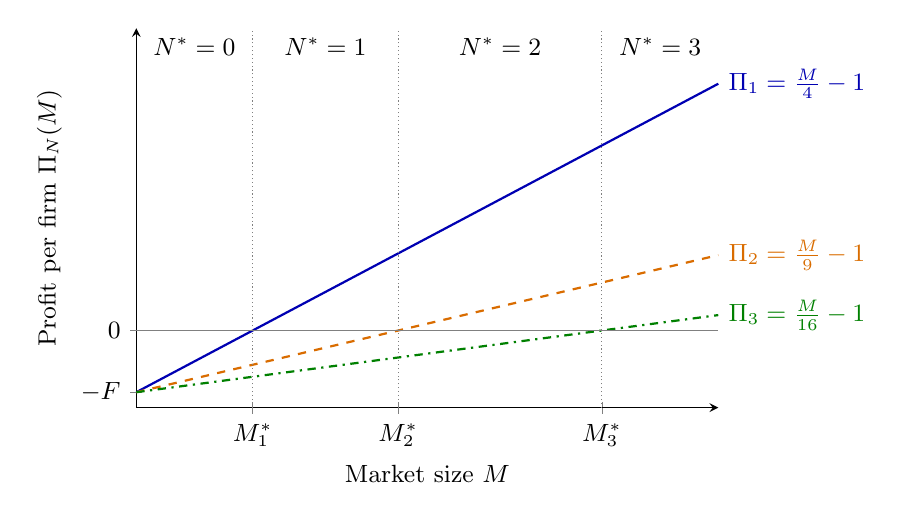
\begin{tikzpicture}
\begin{axis}[
  width=0.74\textwidth, height=6.4cm,
  xmin=0, xmax=20, ymin=-1.25, ymax=4.9,
  axis lines=left,
  clip=false,
  xlabel={Market size $M$}, ylabel={Profit per firm $\Pi_N(M)$},
  xtick={4,9,16}, xticklabels={$M_1^*$, $M_2^*$, $M_3^*$},
  ytick={-1,0}, yticklabels={$-F$, $0$},
  every axis plot/.append style={thick},
  label style={font=\small}, tick label style={font=\small}
]
\addplot[domain=0:20, samples=2, blue!70!black] {x/4 - 1}
  node[pos=1, right, font=\small] {$\Pi_1 = \frac{M}{4} - 1$};
\addplot[domain=0:20, samples=2, orange!85!black, dashed] {x/9 - 1}
  node[pos=1, right, font=\small] {$\Pi_2 = \frac{M}{9} - 1$};
\addplot[domain=0:20, samples=2, green!50!black, dash dot] {x/16 - 1}
  node[pos=1, right, font=\small] {$\Pi_3 = \frac{M}{16} - 1$};
\draw[gray, thin] (axis cs:0,0) -- (axis cs:20,0);
\draw[gray, densely dotted] (axis cs:4,-1.25) -- (axis cs:4,4.9);
\draw[gray, densely dotted] (axis cs:9,-1.25) -- (axis cs:9,4.9);
\draw[gray, densely dotted] (axis cs:16,-1.25) -- (axis cs:16,4.9);
\node[font=\small] at (axis cs:2,4.6) {$N^* = 0$};
\node[font=\small] at (axis cs:6.5,4.6) {$N^* = 1$};
\node[font=\small] at (axis cs:12.5,4.6) {$N^* = 2$};
\node[font=\small] at (axis cs:18,4.6) {$N^* = 3$};
\end{axis}
\end{tikzpicture}
\caption{Entry thresholds under linear Cournot competition (\cref{ex:01-cournot-thresholds}) with the
normalization $\frac{(a - c)^2}{b} = 1$ and $F = 1$. Profit per firm is $\Pi_N = \frac{M}{(N + 1)^2} - 1$.
Each line crosses zero at the threshold $M_N^* = (N + 1)^2$, and the bands show the free-entry number of
firms $N^*$.}
\label{fig:01-thresholds}
\end{figure}

\subsubsection{Bresnahan and Reiss (1991): entry into isolated markets}

\casehead{Question}
How much does entry change competition in a concentrated market? Theories give conflicting answers.
Contestability says that the threat of entry alone disciplines incumbents, while many entry-barrier theories
say that only actual entry matters. \citet{BresnahanReiss1991} propose to measure the effect of each
additional entrant from the relation between market size and the number of firms. The numbers below come
from the working-paper version of the article (Stanford GSB Research Paper 1061).

\casehead{Setting and data}
The sample consists of 202 geographically isolated local markets in the United States.
The typical market is a county seat in the western United States, and the population of the central town
approximates market size. The towns lie at least 25 miles from the nearest town of 1,000 people or more, and
towns within 100 miles of a city of 100,000 are excluded.
Isolation makes it easy to count all competitors. The authors keep only industries whose sellers offer a
narrowly defined product or service and can all be identified. Five survive their data requirements:
doctors, dentists, druggists, plumbers and tire dealers. Firms are counted from telephone books and trade
sources and checked by visits. Practices that share an address and a telephone number count as one firm. In
the sample, mean town population is 3,740, ranging from 120 to 45,090, and the mean number of dentists is
2.6 (working paper, Table~2).
Of the 202 markets, 32 have no dentist, 67 have one and 39 have two (Table~1).

\casehead{Model and estimating equations}
The empirical model generalizes \eqref{eq:01-br-profit} by letting market size, variable profit and fixed
costs depend on observables. The parameter names below are ours, because the paper's symbols clash with the
notation of this book. In market $t$ the profit of each of $N$ firms is
\begin{equation}\label{eq:01-br-latent}
  \Pi_{Nt} = M_t(\lambda)\,V_N(X_t) - F_N(W_t) + u_t .
\end{equation}
The profit shock $u_t$ is standard normal and independent across markets and of the observables. It is common
to all firms in a market. Market size is
\[
  M_t(\lambda) = \mathit{TownPop}_t + \lambda_1 \mathit{NearbyPop}_t + \lambda_2 \mathit{PosGrowth}_t
  + \lambda_3 \mathit{NegGrowth}_t + \lambda_4 \mathit{Commuters}_t ,
\]
with the coefficient on town population normalized to one. The other terms are population within ten miles,
the positive and negative parts of town growth between 1970 and 1980, and residents who commute to work outside
the county. Per-firm variable profit per consumer and fixed costs are
\[
  V_N(X_t) = \eta_1 + X_t\beta^V - \sum_{n=2}^{N}\eta_n ,
  \qquad
  F_N(W_t) = \zeta_1 + \zeta_L W_{Lt} + \sum_{n=2}^{N}\zeta_n ,
\]
The vector $X_t$ contains county demographics such as per capita income. The variable $W_{Lt}$ is the value of
farmland, a proxy for the cost of capital. The parameter $\eta_n$ measures the fall in each firm's variable profit per
consumer when the $n$-th firm enters, and $\zeta_n$ the increase in fixed cost. Because $V_N$ is per firm,
$V_N = \frac{v_N}{N}$ in the notation of \cref{prop:01-entry-thresholds}. Each industry has 19 parameters:
four $\lambda$s, four coefficients in $\beta^V$, five $\eta$s and six $\zeta$s.

\casehead{Estimator}
Write $\bar\Pi_{Nt} = M_t V_N - F_N$ for the deterministic part of profit. The equilibrium number of firms is
$N_t = N$ when $\Pi_{Nt} \ge 0 > \Pi_{N+1, t}$, that is, when $-\bar\Pi_{Nt} \le u_t < -\bar\Pi_{N+1, t}$.
With $\bar\Pi_{1t} \ge \bar\Pi_{2t} \ge \cdots$ and $\Phi$ the standard normal distribution function, this event
has probability
\[
  \Pr(N_t = N) = \Phi\big(-\bar\Pi_{N+1, t}\big) - \Phi\big(-\bar\Pi_{Nt}\big)
               = \Phi\big(\bar\Pi_{Nt}\big) - \Phi\big(\bar\Pi_{N+1, t}\big)
\]
for $N = 1, \dots, 4$. The end categories have $\Pr(N_t = 0) = 1 - \Phi(\bar\Pi_{1t})$ and
$\Pr(N_t \ge 5) = \Phi(\bar\Pi_{5t})$. The parameters maximize the ordered probit log-likelihood
\[
  \ell = \sum_{t} \sum_{N=0}^{5} \indic\{N_t = N\} \ln \Pr(N_t = N \mid M_t, X_t, W_t) .
\]
The authors impose $\bar\Pi_{N+1} \le \bar\Pi_N$ by setting an $\eta_N$ or $\zeta_N$ to zero where necessary. In
the doctors' model, for example, $\eta_3 = \eta_5 = 0$. At the sample means of the covariates, the entry
thresholds are
\begin{equation}\label{eq:01-br-threshold}
  M_N^* = \frac{\zeta_1 + \zeta_L \bar W_L + \sum_{n=2}^{N}\zeta_n}{\eta_1 + \bar X\beta^V - \sum_{n=2}^{N}\eta_n} ,
\end{equation}
the market size at which $\bar\Pi_N = 0$, and the per-firm thresholds are $\tau_N = \frac{M_N^*}{N}$.

\casehead{Identification}
Market size is the excluded variable. It multiplies variable profit and leaves fixed costs unchanged, so the
way the distribution of $N_t$ shifts with population traces out the thresholds. The normalizations fix the
units of market size (town residents) and the scale of profit (unit variance of $u_t$). The thresholds are
ratios, so they do not depend on the scale normalization. The parameters $\eta_n$ and $\zeta_n$ are
separately identified only because $\eta_n$ interacts with market size and $\zeta_n$ does not. In practice
the data barely separate falling variable profits from rising fixed costs, and many individual estimates have
large standard errors (working paper, pp.~16 and 20). The thresholds depend only on the ratio of fixed costs
to variable profits, and restricting the cost parameters changes them little (working paper, p.~21). Five
assumptions are maintained. Firms within an industry differ only through the entry-order terms $\eta_n$ and
$\zeta_n$, and one profit shock is common to all firms in a market. Population is exogenous to the number of firms, and isolation captures every competitor. Markets
are in long-run equilibrium. With a single cross-section, sunk and fixed costs cannot be distinguished (working
paper, fn.~5).

\casehead{Main results}
\Cref{tab:01-br-thresholds} reproduces the estimated thresholds. A monopoly tire dealer or druggist needs about
500 people in town, and a monopoly doctor or dentist between 700 and 900. A monopoly plumber needs about
1,430 people, twice the dentist threshold and 1.6 times the doctor threshold (\cref{tab:01-br-thresholds}).
The per-firm ratios decline with $N$. For doctors, dentists, druggists and tire dealers, the second firm needs
roughly 1.8 to 2.0 times the customers of a monopolist, while plumbers' ratios stay near one throughout.
For the third firm the ratio is near one for doctors and plumbers (1.10 and 1.00), 1.28 for tire dealers and
1.58 for druggists. For dentists Table~4 prints 0.79, while the printed thresholds imply 1.10.
For the fourth and fifth firms the ratios lie between 0.94 and 1.14 in every industry, so the decline stops
abruptly after the first few entrants.
Likelihood ratio tests cannot reject $\tau_3 = \tau_4 = \tau_5$ except for dentists. They reject
$\tau_1 = \cdots = \tau_5$ in all five industries, so the variation in the first two thresholds is not
sampling noise. \Cref{fig:01-br-ratios} redraws the paper's Figure~4, which plots $\frac{\tau_5}{\tau_N}$
against $N$.

\begin{table}[htbp]
\centering
\caption{Entry thresholds in five retail and professional industries}
\label{tab:01-br-thresholds}
\small
\setlength{\tabcolsep}{4.5pt}
\begin{tabular}{@{}l rrrrr rrrr@{}}
\toprule
\multicolumn{10}{@{}l}{\textit{Panel A. Thresholds and per-firm threshold ratios}} \\
\addlinespace[2pt]
 & \multicolumn{5}{c}{Threshold $M_N^*$ (thousands)} & \multicolumn{4}{c}{Ratio $\frac{\tau_{N+1}}{\tau_N}$} \\
\cmidrule(lr){2-6}\cmidrule(l){7-10}
Industry & $N = 1$ & $2$ & $3$ & $4$ & $5$ & $\frac{\tau_2}{\tau_1}$ & $\frac{\tau_3}{\tau_2}$ & $\frac{\tau_4}{\tau_3}$ & $\frac{\tau_5}{\tau_4}$ \\
\midrule
Doctors      & 0.88 & 3.49 & 5.78 & 7.72 & 9.14 & 1.98 & 1.10 & 1.00 & 0.95 \\
Dentists     & 0.71 & 2.54 & 4.18 & 5.43 & 6.41 & 1.78 & 0.79 & 0.97 & 0.94 \\
Druggists    & 0.53 & 2.12 & 5.04 & 7.67 & 9.39 & 1.99 & 1.58 & 1.14 & 0.98 \\
Plumbers     & 1.43 & 3.02 & 4.53 & 6.20 & 7.47 & 1.06 & 1.00 & 1.02 & 0.96 \\
Tire dealers & 0.49 & 1.78 & 3.41 & 4.74 & 6.10 & 1.81 & 1.28 & 1.04 & 1.03 \\
\bottomrule
\end{tabular}

\medskip
\begin{tabular}{@{}l rr rr rr rr@{}}
\toprule
\multicolumn{9}{@{}l}{\textit{Panel B. Likelihood ratio tests of equal per-firm thresholds}} \\
\addlinespace[2pt]
 & \multicolumn{2}{c}{$\tau_4 = \tau_5$} & \multicolumn{2}{c}{$\tau_3 = \tau_4 = \tau_5$}
 & \multicolumn{2}{c}{$\tau_2 = \cdots = \tau_5$} & \multicolumn{2}{c}{$\tau_1 = \cdots = \tau_5$} \\
\cmidrule(lr){2-3}\cmidrule(lr){4-5}\cmidrule(lr){6-7}\cmidrule(l){8-9}
Industry & LR & df & LR & df & LR & df & LR & df \\
\midrule
Doctors      & 1.12 & 1 & 6.20      & 3 & 8.33      & 4 & 45.06$^*$  & 6 \\
Dentists     & 1.59 & 1 & 12.30$^*$ & 2 & 19.13$^*$ & 4 & 36.67$^*$  & 5 \\
Druggists    & 0.43 & 2 & 7.13      & 4 & 65.28$^*$ & 6 & 113.92$^*$ & 8 \\
Plumbers     & 1.99 & 2 & 4.01      & 4 & 12.07     & 6 & 15.62$^*$  & 7 \\
Tire dealers & 3.59 & 2 & 4.24      & 3 & 14.52$^*$ & 5 & 20.89$^*$  & 7 \\
\bottomrule
\end{tabular}
\par\smallskip
\begin{minipage}{\textwidth}\footnotesize
\textit{Notes:} Thresholds are evaluated at sample means with \eqref{eq:01-br-threshold}, using the baseline
ordered probit estimates, and are measured in thousands of people. The per-firm threshold is $\tau_N = \frac{M_N^*}{N}$. Ratios are as printed in the
source. The printed thresholds imply $\frac{\tau_3}{\tau_2} = 1.10$ for dentists, and all other ratios match
the thresholds up to rounding. In Panel B, LR is the likelihood ratio statistic and df its degrees of
freedom. An asterisk marks a statistic above the 5 percent cutoff of the chi-squared distribution with the
stated degrees of freedom. Source: Bresnahan and Reiss (1991), Table~4
(working-paper version, Research Paper 1061).
\end{minipage}
\end{table}

\begin{figure}[htbp]
\centering
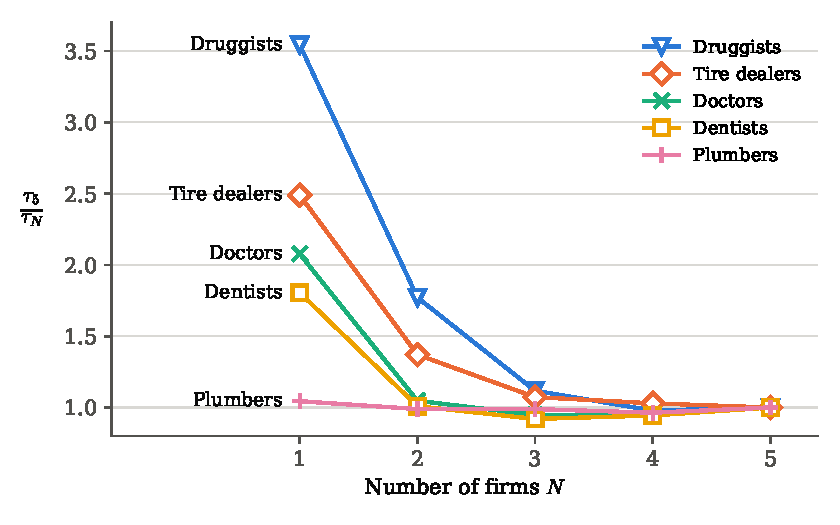
\includegraphics[width=0.82\textwidth]{figures/ch01/br_threshold_ratios.pdf}
\caption{Ratio of the per-firm threshold for five firms to the per-firm threshold for $N$ firms,
$\frac{\tau_5}{\tau_N}$, by industry. A value near one means that the $N$-th firm needs about as many customers
as the fifth. From $N = 3$ on, the ratios lie between 0.92 and 1.12 in every industry. Redrawn from the thresholds in \cref{tab:01-br-thresholds}. Source: Bresnahan and Reiss (1991),
Figure~4 (working-paper version).}
\label{fig:01-br-ratios}
\end{figure}

\casehead{Robustness}
Using ``four or more firms'' as the top category extends the analysis to eight industries. The thresholds of
the original five change little, and heating contractors and barbers show the same pattern. Auto dealers are
the exception, with a per-firm ratio for the fourth dealer well above one (working paper, pp.~18--19). The authors attribute this to product differentiation. Most dealer triopolies pit the three
domestic manufacturers against one another, and the fourth dealer is typically the first intrabrand
competitor. The hypothesis of equal fixed costs across entrants is rejected for every industry except
plumbers, but imposing it barely moves the thresholds. Restricting the sample to very isolated markets, at least 40 miles
from the next town of 1,000 people, leaves 157 markets and similar ratios.
Treating every county with fewer than 10,000 residents in 1980 as a market, isolated or not, sharply reduces
the estimated effect of the second and third doctors and dentists. This is what we would expect if customers
in less isolated towns shop elsewhere, and it supports the strict market definition.

\casehead{Interpretation}
Under the maintained hypotheses that firms in each industry offer similar services with similar technologies
and costs, the results say that entry beyond the third firm changes margins very little. Most of the
competitive effect of entry is felt in highly concentrated markets, with the second and third entrants. The
authors were surprised. They had expected margins, or entry barriers, to erode gradually. Through the lens of
\cref{ex:01-cournot-thresholds} the pattern is sharper than linear Cournot competition implies. Cournot
predicts a second-firm ratio of $1.125$ and ratios above one for every later entrant. Four of the industries
instead show second-firm ratios between 1.78 and 1.99, and every industry shows ratios close to one from the
fourth firm on. In the words of Einav and Levin, competition
appears to ``kick in relatively quickly'' with just a few firms and then does not ramp up with further entry
(p.~155).

\casehead{Critiques}
Bresnahan and Reiss list the main caveats themselves. Without prices, quantities and the timing of entry, they
cannot say whether markets with three or more firms are competitive, only that conduct stops changing
(\cref{rem:01-etr-meaning}). Ratios above one can reflect costlier later entrants as well as falling margins
(\cref{rem:01-etr-costs}). Professionals with low opportunity costs might seek out isolated monopolies, which
would raise the monopoly ratios for reasons unrelated to competition. Einav and Levin add a critique of the
literature that followed (pp.~155--156). One might have expected researchers to look for other identifying
variation, such as differences in fixed costs or entry restrictions, or to gather data on prices and costs.
Instead, most follow-up work developed econometric methods that allow firm heterogeneity or relax parametric
restrictions \citep{Berry1992,BerryTamer2006}, often applying the original identifying assumptions where they
are less compelling. This produced a rich literature on identification and estimation that has not
necessarily brought us closer to the original question.

\casehead{Contribution}
The paper shows how sparse data, used with theory and a clean design, can answer an important question. Counts
of firms in markets of different sizes reveal how competition varies with the number of firms. The entry model
gets around missing data on prices and quantities, which is one reason it has been so influential (p.~160). It
also reframes the SCP question. Concentration is treated as an equilibrium outcome driven by an exogenous
shifter, market size, and the relation between the two identifies how conduct changes with structure.

\begin{remark}[Market size and concentration]\label{rem:01-sutton}
If the per-firm thresholds converge to a finite limit $\tau_\infty$, concentration vanishes in large markets.
Because $\tau_N$ is nondecreasing, $M < M^*_{N^*+1} = (N^* + 1)\tau_{N^*+1} \le (N^* + 1)\tau_\infty$ by
\cref{prop:01-entry-thresholds}(iii). Hence $N^* > \frac{M}{\tau_\infty} - 1$, which grows without bound with
$M$. This argument treats fixed costs as exogenous. \citet{Sutton1991} shows that the conclusion fails when
firms can raise demand through sunk outlays such as advertising or research and development. Such
endogenous sunk costs escalate with market size, and concentration can stay bounded away from zero
however large the market becomes.
\end{remark}

\subsubsection{Industry dynamics}

Many questions about market structure are dynamic \citep[p.~156]{EinavLevin2010}. Do new industries follow a
common life cycle of entry and consolidation? How do firm and industry growth vary with market
characteristics? Are mergers followed quickly by entry, and how do industries adapt to booms and recessions?
A dynamic view can also temper static intuition. Higher concentration reduces static welfare, but the prospect
of market power can create strong incentives to innovate.

The literature has two strands (p.~156). The first looks across industries for robust patterns of survival,
turnover and growth. Its main finding is the large heterogeneity across establishments even within narrow
industries. This finding shaped theoretical models of industry dynamics \citep{Hopenhayn1992}, which in turn
inspired work on firm heterogeneity in international trade \citep{Melitz2003}. The link between entry, exit and
firm characteristics also entered the study of productivity through \citet{OlleyPakes1996}. The second strand
builds models of dynamic equilibrium in single industries, often in the framework of \citet{EricsonPakes1995}.
\citet{Benkard2004} applies such a model to commercial aircraft, where learning by doing lowers costs
dramatically. Equilibrium prices can lie below marginal cost early in a product's life, because extra output
speeds learning. The prospect of market power is what motivates firms to move down the learning curve.
Consumers gain from lower prices both early on and later, when costs are lower. Newer methods estimate sunk
costs, learning and adjustment frictions from panel data on firms or local markets
\citep{AguirregabiriaMira2007,BajariBenkardLevin2007,PakesOstrovskyBerry2007}. \citet{AguirregabiriaCollardWexlerRyan2021}
survey this work in Volume~4 of the Handbook of Industrial Organization. Their chapter lays out the Markov
perfect equilibrium framework, the data typically available, identification and estimation, and applications to
innovation, mergers, regulation, investment, advertising and dynamic pricing \citep[Preface, pp.~xvi--xvii]{HoHortacsuLizzeri2021}.

\begin{remark}[Why learning can push prices below marginal cost]\label{rem:01-learning}
A two-period monopolist faces demand $Q(p)$ in each period and discounts the future by a factor $\delta$. The
first-period cost is $c_1$. Learning makes the second-period cost $c_2(Q_1)$ fall with first-period output,
so $c_2' < 0$. Let $\pi_2(c_2)$ be the optimal second-period profit. By the envelope theorem
$\pi_2'(c_2) = -q_2$, where $q_2$ is second-period output. The firm chooses $p_1$ to maximize
$(p_1 - c_1)Q(p_1) + \delta\,\pi_2\big(c_2(Q(p_1))\big)$. The first-order condition is
\[
  Q(p_1) + (p_1 - c_1)Q'(p_1) + \delta\,\pi_2'(c_2)\,c_2'(Q_1)\,Q'(p_1) = 0 .
\]
Substituting $\pi_2' = -q_2$ and dividing by $-Q'(p_1) > 0$ gives
\[
  p_1 = \big(c_1 - \delta q_2 \lvert c_2' \rvert\big) - \frac{Q(p_1)}{Q'(p_1)} .
\]
The firm prices off an effective marginal cost that is lower than $c_1$ by the discounted value of learning. If
learning is strong enough, $p_1 < c_1$.
\end{remark}

The data available for such models often pale in comparison with the ambitious questions asked, so researchers
fill the gaps with strong assumptions (p.~156). Einav and Levin view this work as ``a quantitative theory
exercise'' (pp.~156--157). It sheds light on dynamic competition in a model with reasonable parameter values.
They do not see this as a problem. It is hard to imagine a clean research design that could pin down the
long-run effect on innovation of a change in the patent system. When the entire history of an industry is a
single data point, quasi-experimental variation is rare, and models are the only way to study such
questions.

\subsection{Structural and design-based approaches}\label{sec:01-today-debate}

Thirty years ago empirical IO resembled other applied fields \citep[p.~157]{EinavLevin2010}. Industrial
organization economists ran cross-industry regressions and faced endogeneity, omitted variables and reverse
causality, much as labor economists running wage regressions did. Since then IO has moved in a distinctive
direction. It turned toward single industries, where measurement and identification are cleaner, and toward
analyses framed by an economic theory of the industry. In the same journal issue, \citet{AngristPischke2010}
describe a parallel move in applied microeconomics toward randomized experiments and quasi-experiments. They
also criticize empirical IO, and Einav and Levin reply. The exchange clarifies the stance of this book.

\subsubsection{Clean measurement versus the object of interest}

No one disagrees about the ideal (p.~157). Every researcher would like to define an object of interest and
then design the perfect experiment to measure it. Without that ideal, researchers face trade-offs, and a
common one is between the cleanness of a measurement and how well the measured object proxies for the object
of interest. Einav and Levin illustrate it with cereal (pp.~157--158). Suppose the object of interest is the
$J \times J$ matrix of price elasticities $E = [\varepsilon_{jk}]$.

\begin{itemize}
  \item The standard IO approach controls for shifts in demand and assumes that the remaining correlation of
        prices across cities reflects costs, as with the Hausman instruments of \citet{Nevo2001}. Within the
        demand model this identifies all of $E$. The assumption may fail.
  \item A design-based alternative looks for an episode that moved one price for an explicable and plausibly
        exogenous reason. An example would be a week in which the pricing algorithm for Froot Loops
        malfunctioned and produced an unintended sale. Such an episode credibly identifies one column of
        $E$, the responses $\varepsilon_{j,\mathrm{FL}}$ of all products to the price of Froot Loops. To learn
        the rest of $E$ we must extrapolate, for instance by assuming that a change in the price of Frosted
        Flakes, or of any cereal, would have analogous effects.
\end{itemize}

Neither approach is ideal. The first relies on a questionable identifying assumption but frames the exercise
directly in terms of the object of interest. The second measures a few entries convincingly but reaches the
object of interest only through a questionable extrapolation. Einav and Levin argue that evaluating entire
research approaches in the abstract paints too simple a picture (p.~158). The right resolution depends on the
question, the data and how compelling a rationale theory provides for the assumptions. There is room for many
approaches, even to the same question, and careful work from different angles is often complementary.

\subsubsection{Theory, transparency and mechanisms}

Angrist and Pischke favor measurement strategies uncontaminated by restrictions from an economic model, partly
on grounds of transparency. Einav and Levin call the implied link between theory and obscurity ``a false
equivalence'' (p.~158). A model derived from theory can be exposited with perfect clarity, and a linear
regression can be exposited with perfect obscurity. It is more natural to start with a research question and
ask how much theory can say about it. Standard theory says little about student behavior in third-grade
classrooms, the setting of Angrist and Pischke's class-size example. There a statistical approach that exploits
variation across thousands of roughly parallel classrooms is attractive. Industrial organization is largely
about firms and markets, which is the other side of the contrast quoted in \cref{sec:01-what-is-io}
(pp.~158--159). Moreover, the interesting question is often a mechanism rather than a single
causal effect. Markets differ greatly, so importing particular numbers across markets is rarely compelling.
Empirical work generalizes best by building support for principles of strategic interaction and market
functioning that apply across industries.

\subsubsection{The merger example}

Angrist and Pischke chose merger evaluation as their example. They dismiss merger simulation as needlessly
indirect and ask why there has not been more retrospective analysis of past mergers. Einav and Levin answer
that the point is good at one level and misses the point at another (p.~159). If the Department of Justice had
to review a merger of Microsoft and Yahoo!, the price effects of past airline or office-supply mergers would be
of little use. It is far more useful to lay out a clear framework for the potential effects of that merger and
to add the best available evidence. \Cref{ch:mergers} presents retrospective studies and merger simulations
side by side, and it shows how each disciplines the other.

The bottom line is that economic theory and the search for compelling identifying variation are allies
(p.~159). The applied work that Einav and Levin find most exciting rests on careful measurement from data with
good variation and then frames the analysis in a coherent economic model. The model gives a way to think about
how the industry works and, potentially, to draw conclusions about policy or general principles. The case
studies of this book are chosen and presented with that standard in mind.

\subsubsection{Methods, applications and the questions IO asks}

Einav and Levin also voice concerns about the field itself (pp.~159--160). Their main concern is that too
little effort goes into compelling applications relative to new econometric methods. Better methods are
valuable if they are eventually used in compelling ways and do not become an end in themselves. In demand
estimation, researchers may have tolerated imperfect price variation because the main contribution was a
method that applies more broadly. Data limitations explain part of the current balance. Some of the most
influential methods were responses to scarce data. The entry model of \citet{BresnahanReiss1991} gets around
missing data on prices and quantities, and the demand model of \citet{BerryLevinsohnPakes1995} needs only
market-level data. As firms collect vast amounts of data on customers, prices, quantities and locations,
richer data may substitute for methods and shift effort toward applications.

A related danger applies to all empirical strategies: the elegance of a solution can pull researchers toward
less important questions (p.~160). Einav and Levin use eBay as an example. Viewed as a laboratory for elegant
auction methods, eBay invites the study of ever narrower submarkets. Broader questions, such as why eBay
succeeded as an institution or how it competes with Amazon and other platforms, would then go unasked.
Researchers should ``resist the temptation of grabbing a hammer and letting it pull them toward a limited set
of nails'' (p.~160).

The last concern is about scope. Schmalensee's review of the cross-industry literature concluded that it had
taught us little about how markets work (\cref{sec:01-scp-today}). After two decades of industry studies, we know a
lot about specific industries such as automobiles, airlines, electricity, and cement and concrete. This
knowledge is extremely disaggregated and does not easily accumulate across industries. As a result, IO has
ceded many important questions about the overall organization of production to trade and macroeconomics.
Einav and Levin suggest that ``it may be time to reclaim them'' (p.~160). The debate over rising markups in
\cref{sec:01-rising-markups} is one place where IO economists are doing so, and it shows how hard the
cross-industry questions remain.

\section{Roadmap of the book}\label{sec:01-roadmap}

The book has four parts and three appendices. Every chapter follows the order of this introduction: theory in
general form first, then case studies that show how the theory meets data. \Cref{tab:01-roadmap} lists, for
each chapter, its central question, its main models and tools, and the papers it treats as full case studies.
Readings that are not case studies receive shorter treatments in the same chapters.

\subsection{The four parts}

Part~I treats market power, its theory and its measurement. This chapter introduced the questions, the SCP
tradition and its failure, the NEIO response and the structural workflow. \Cref{ch:theory} develops the theory that the
rest of the book uses. It covers monopoly pricing, Cournot and Bertrand competition, conjectural variations and
the conduct parameter, pass-through and welfare. \Cref{ch:conduct} asks whether market power can be detected
and measured in homogeneous-good industries. It covers tax pass-through tests, the Panzar-Rosse statistic,
residual demand, the identification of conduct by demand rotations, and direct validations against cost data.
\Cref{ch:diffprod} turns to differentiated products. It derives multi-product Bertrand pricing and diversion
ratios, discusses existence and uniqueness of equilibrium, and contrasts product space with characteristic
space.

Part~II is about demand estimation. \Cref{ch:aids} estimates demand in product space with the Almost Ideal
Demand System, multi-stage budgeting and Hausman instruments. \Cref{ch:discrete} builds the foundations of
discrete choice, including the vertical model and the pure characteristics model. \Cref{ch:logit} covers the
logit and nested logit, the Berry inversion and instruments for price. \Cref{ch:blp} develops the random
coefficients logit of Berry, Levinsohn and Pakes, its estimation and its supply side. \Cref{ch:airlines}
applies these tools to airline hubs and entry. \Cref{ch:newgoods} measures the value of new goods and the bias
in price indexes that ignore them.

Part~III is about competition policy. \Cref{ch:mergers} covers horizontal mergers. It treats market
definition, the theory of mergers in Cournot and differentiated-product models, upward pricing pressure,
merger simulation and retrospective studies. \Cref{ch:collusion-theory} develops the theory of collusion in
repeated games, with demand fluctuations, imperfect monitoring, private information and communication.
\Cref{ch:collusion-evidence} studies how real cartels operated and how collusion can be detected in prices and
bids.

Part~IV is about auctions. \Cref{ch:auction-theory} develops the theory of single-object auctions, from
independent private values to the affiliated values model of Milgrom and Weber. \Cref{ch:auction-empirics}
asks what bid data reveal about values and costs. It covers identification, the estimator of Guerre, Perrigne
and Vuong, unobserved heterogeneity and entry.

Three appendices support the main text. \Cref{app:econometrics} collects the econometric tools: instrumental variables, the
generalized method of moments, maximum likelihood and simulation estimators, the delta method, nonparametric
estimation, and event studies. \Cref{app:math} collects the mathematical tools: the envelope and implicit
function theorems, duality, extreme value algebra, order statistics, contraction mappings, log-concavity and
affiliation. \Cref{app:problems} contains worked problems with full solutions. Two simulated markets recur
there as running examples. One has 25 logit products sold by five owners. The other has 100 markets drawn from a pool of ten
products, and each market offers between four and nine of them. It is generated from a random-coefficients logit
with a cost shifter, and on it the vertical, logit and random-coefficients estimators are compared.

\begin{table}[htbp]
\centering
\caption{Roadmap of the book}
\label{tab:01-roadmap}
\scriptsize
\renewcommand{\arraystretch}{1.0}
\begin{tabularx}{\textwidth}{@{}>{\raggedright\arraybackslash}p{1.95cm}
  >{\raggedright\arraybackslash}X >{\raggedright\arraybackslash}X >{\raggedright\arraybackslash}X@{}}
\toprule
Chapter & Central question & Main models and tools & Case studies in depth \\
\midrule
\multicolumn{4}{@{}l}{\textit{Part I. Market power: theory and measurement}} \\
\ref{ch:intro}. Introduction & How do we learn about market power and its causes? & SCP regressions, the
  Cournot link between margins and concentration, the conduct parameter, the structural workflow &
  \citet{BresnahanReiss1991}, \citet{GriecoMurryYurukoglu2024} (and substantive treatments of
  \citet{Bresnahan1989} and \citet{EinavLevin2010}) \\
\ref{ch:theory}. Pricing theory & How do demand, cost and conduct determine prices? & Monopoly pricing,
  Cournot and Bertrand oligopoly, conjectural variations, pass-through, welfare & None \\
\ref{ch:conduct}. Measuring market power & Can we detect and measure market power with homogeneous goods? &
  Tax pass-through tests, Panzar-Rosse statistic, residual demand, identification of conduct by rotations &
  \citet{Sumner1981}, \citet{Corts1999}, \citet{GenesoveMullin1998}, \citet{Wolfram1999} \\
\ref{ch:diffprod}. Differentiated oligopoly & How do multi-product firms price differentiated goods? &
  Multi-product Bertrand-Nash pricing, ownership matrix, diversion ratios, existence and uniqueness, location
  models & None \\
\addlinespace
\multicolumn{4}{@{}l}{\textit{Part II. Demand estimation}} \\
\ref{ch:aids}. AIDS & How do we estimate flexible demand in product space? & Duality, AIDS, multi-stage
  budgeting, Hausman instruments, welfare & \citet{DeatonMuellbauer1980a}, \citet{HausmanLeonardZona1994},
  \citet{ChaudhuriGoldbergJia2006} \\
\ref{ch:discrete}. Discrete choice & How do individual choices aggregate to market demand? & Random utility,
  vertical model, pure characteristics model, hedonic approach & \citet{Bresnahan1987},
  \citet{BerryPakes2007} \\
\ref{ch:logit}. Logit & How do we estimate logit demand with endogenous prices? & Logit, Berry inversion,
  instruments, nested logit & \citet{Berry1994}, \citet{Einav2007}, \citet{Hendel1999} \\
\ref{ch:blp}. BLP & How do we obtain realistic substitution from market-level data? & Random coefficients
  logit, contraction mapping, GMM, supply side, micro moments & \citet{BerryLevinsohnPakes1995},
  \citet{Nevo2000a}, \citet{Nevo2001}, \citet{BerryLevinsohnPakes2004}, \citet{Goldberg1995} \\
\ref{ch:airlines}. Airlines & Why are fares high at hubs, and how does entry discipline them? & Fare
  regressions, event studies, discrete choice with consumer types and hub costs & \citet{Borenstein1989},
  \citet{WhinstonCollins1992}, \citet{BerryCarnallSpiller2006} \\
\ref{ch:newgoods}. New goods & What is a new good worth to consumers? & Virtual prices, compensating variation,
  logit welfare, micro moments & \citet{Hausman1997}, with the comment by \citet{Bresnahan1997};
  \citet{Trajtenberg1989}, \citet{Petrin2002}, \citet{Gentzkow2007} \\
\addlinespace
\multicolumn{4}{@{}l}{\textit{Part III. Competition policy}} \\
\ref{ch:mergers}. Mergers & When do horizontal mergers raise prices? & Market definition, Cournot merger
  analysis, upward pricing pressure, merger simulation, retrospectives & \citet{FarrellShapiro1990},
  \citet{FarrellShapiro2010}, \citet{Nevo2000b}, \citet{BjornerstedtVerboven2016},
  \citet{MillerWeinberg2017} \\
\ref{ch:collusion-theory}. Collusion: theory & How can firms sustain collusion without enforceable contracts? &
  Repeated games, optimal punishments, demand fluctuations, imperfect monitoring, private information,
  communication & \citet{GreenPorter1984}, \citet{RotembergSaloner1986},
  \citet{AtheyBagwellSanchirico2004}, \citet{HarringtonSkrzypacz2011} \\
\ref{ch:collusion-evidence}. Collusion: evidence & How did cartels operate, and how can we detect them? &
  Regime-switching supply relations, tests of price-war theories, bidding rings, tests for bid rigging &
  \citet{Porter1983}, \citet{Ellison1994}, \citet{PorterZona1993}, \citet{Asker2010} \\
\addlinespace
\multicolumn{4}{@{}l}{\textit{Part IV. Auctions}} \\
\ref{ch:auction-theory}. Auction theory & How do rules and information shape bids and revenue? & Private and
  affiliated values, first- and second-price equilibrium, revenue equivalence, reserve prices, linkage
  principle & \citet{MilgromWeber1982} \\
\ref{ch:auction-empirics}. Auction empirics & What do bids reveal about values and costs? & Order-statistic
  inversion, the GPV estimator, unobserved heterogeneity, entry, timber auctions &
  \citet{AtheyHaile2002}, \citet{AtheyHaile2007}, \citet{GuerrePerrigneVuong2000},
  \citet{Krasnokutskaya2011}, \citet{AtheyLevinSeira2011} \\
\bottomrule
\end{tabularx}
\par\smallskip
\begin{minipage}{\textwidth}\footnotesize
\textit{Notes:} The last column lists the papers treated as full case studies, following the structure
described in \cref{sec:01-roadmap-conventions}. Each chapter also gives shorter treatments of the other
readings in its scope.
\end{minipage}
\end{table}

\subsection{Reading paths}

The chapters build on one another, but several shorter paths through the book work well.
\begin{itemize}
  \item A reader interested in antitrust and merger analysis can read
        \cref{ch:theory,ch:conduct,ch:diffprod,ch:logit,ch:blp,ch:mergers}. This path runs from pricing
        theory and the measurement of market power to the demand models that merger simulation requires.
  \item A reader interested in demand estimation can read
        \cref{ch:aids,ch:discrete,ch:logit,ch:blp,ch:airlines,ch:newgoods}, after \cref{sec:01-workflow} and
        the multi-product pricing of \cref{ch:diffprod}.
  \item A reader interested in collusion can read
        \cref{ch:theory,ch:conduct,ch:collusion-theory,ch:collusion-evidence}.
  \item A reader interested in auctions can read \cref{ch:auction-theory,ch:auction-empirics}, after
        \cref{sec:01-today-auctions}. The bid-rigging material of \cref{ch:collusion-evidence} is a natural
        complement.
\end{itemize}

\subsection{Prerequisites and conventions}\label{sec:01-roadmap-conventions}

We assume graduate training in microeconomic theory and econometrics. On the theory side the reader should
know consumer theory and duality, and Nash, subgame perfect and Bayesian Nash equilibrium. On the econometric
side the reader should know least squares, instrumental variables, the generalized method of moments and
maximum likelihood. \Cref{app:econometrics,app:math} fill gaps. For the theory of industrial organization at
greater length, \citet{Tirole1988} remains the standard reference. For surveys of recent work, including topics
outside this edition, the reader can turn to Volumes~4 and~5 of the Handbook of Industrial Organization
\citep{HoHortacsuLizzeri2021a,HoHortacsuLizzeri2021}. Their Preface describes every chapter
\citep[pp.~xv--xxi]{HoHortacsuLizzeri2021}. The first five chapters review econometric methods that continue the
NEIO program, Chapters~6 to~9 review theory, and Chapters~10 to~17 apply both to policy questions and to
particular sectors. \Cref{tab:01-handbook} lists the chapters and the parts of this book that each one extends.

\begin{table}[htbp]
\centering
\caption{The chapters of the Handbook of Industrial Organization, Volumes 4 and 5}
\label{tab:01-handbook}
\footnotesize
\renewcommand{\arraystretch}{1.08}
\begin{tabularx}{\textwidth}{@{}>{\raggedright\arraybackslash}p{1.1cm}
  >{\raggedright\arraybackslash}p{4.4cm} >{\raggedright\arraybackslash}X >{\raggedright\arraybackslash}p{3.3cm}@{}}
\toprule
Chapter & Authors & Topic & Extends \\
\midrule
\multicolumn{4}{@{}l}{\textit{Volume 4: econometric methods (Chapters 1 to 5) and theory (Chapters 6 to 9)}} \\
1 & Berry and Haile & Foundations of demand estimation & \cref{ch:discrete,ch:logit,ch:blp} \\
2 & Gandhi and Nevo & Demand and supply in differentiated-products industries, opening with
  \citet{Bresnahan1987} & \cref{ch:discrete,ch:blp,ch:mergers} \\
3 & De Loecker and Syverson & Productivity, and the production approach to market power &
  \cref{sec:01-rising-markups} \\
4 & Aguirregabiria, Collard-Wexler and Ryan & Dynamic games & \cref{sec:01-today-structure} \\
5 & Kline, Pakes and Tamer & Moment inequalities and partial identification & \cref{sec:01-today-structure} \\
6 & Gavazza and Lizzeri & Frictions in product markets & Not covered \\
7 & Jullien, Pavan and Rysman & Two-sided markets, pricing and network effects & \cref{sec:01-early-studies} \\
8 & Bergemann and Ottaviani & Information markets and nonmarkets & Not covered \\
9 & Lee, Whinston and Yurukoglu & Contracting in vertical markets & Not covered \\
\addlinespace
\multicolumn{4}{@{}l}{\textit{Volume 5: applications to policy questions and sectors}} \\
10 & Agarwal and Budish & Market design & \cref{ch:auction-theory} \\
11 & Horta{\c{c}}su and Perrigne & Empirical perspectives on auctions & \cref{ch:auction-empirics} \\
12 & Asker and Nocke & Collusion, mergers and related antitrust issues &
  \cref{ch:mergers,ch:collusion-theory,ch:collusion-evidence} \\
13 & Bryan and Williams & Innovation: market failures and public policies & Not covered \\
14 & Einav, Finkelstein and Mahoney & Selection markets & \cref{sec:01-today-pricing} \\
15 & Clark, Houde and Kastl & Financial markets & Not covered \\
16 & Handel and Ho & Health care markets & \cref{sec:01-scp-today} \\
17 & Kellogg and Reguant & Energy and environmental markets & \cref{sec:01-today-auctions} \\
\bottomrule
\end{tabularx}
\par\smallskip
\begin{minipage}{\textwidth}\footnotesize
\textit{Notes:} Chapter titles are abbreviated. ``Extends'' names the chapter or section of this book that the
Handbook chapter continues. Source: \citet[Preface, pp.~xv--xxi]{HoHortacsuLizzeri2021}.
\end{minipage}
\end{table}

Notation is fixed across chapters. Markets are indexed by $t$ and products by $j$, with $j = 0$ the outside
good. Firms are indexed by $f$ in differentiated-product models and by $i$ in homogeneous-good models, and
consumers by $i$ in discrete choice models. Market shares are $s_{jt}$, marginal costs $mc_{jt}$, the price elasticity of demand
$\varepsilon > 0$, the conduct parameter $\theta$ and the ownership matrix $\Omega$. Mean utility is
$\delta_{jt} = x_{jt}\beta - \alpha p_{jt} + \xi_{jt}$, and auctions use $v$ for values, $b$ for bids and $G$
for the distribution of bids. When a chapter must depart from this notation, or rename the symbols of a paper,
it says so at first use.

Each case study follows the same order. We state the economic question and why it matters, the institutional
setting and the data. We then write the model and the exact estimating equations, the estimator, the
instruments and the identification argument. We reproduce the key results in a table, citing the table number
in the original paper, and discuss robustness, interpretation, the critiques raised in the literature and the
paper's contribution. Every chapter ends with exercises and with bibliographic notes that place its papers in
context.
